\documentclass{standalone}
\usepackage{standalone}

\begin{document}
\section{Naive Minimizer Approach}
Minimizer is described enough above in the Basics section. We ran a W length window over the whole reference genome and stored the K length minimizers which could cover consecutive windows. By the term Consecutive Windows, we meant a set of windows where each window's starting position has starting position difference one with at least one other window in the set. We would only store the position of the first occurrence of the minimizer in the consecutive windows along with the lowest starting position and highest ending position among the windows. We would map this kind of triplets to the corresponding minimizer with the help of unordered map for better efficiency. For making the program more efficient in perspective of time and memory, we have stored minimizer converting it to an integer.

Then we took windows from reads and find it in the unordered map converting to integer for being compatible. On the other experiment, we have done only taking K-mers instead of window or minimizer. In the last version, this idea survived. In Figure \ref{fig:naive_min}, there are four minimizers found in different positions of the reference. In the read which positions could not be matched are shown in gray color.
Minimap\cite{minimap} also used this technique with some enhancement in their tool.
\begin{figure}
	\centering
	
	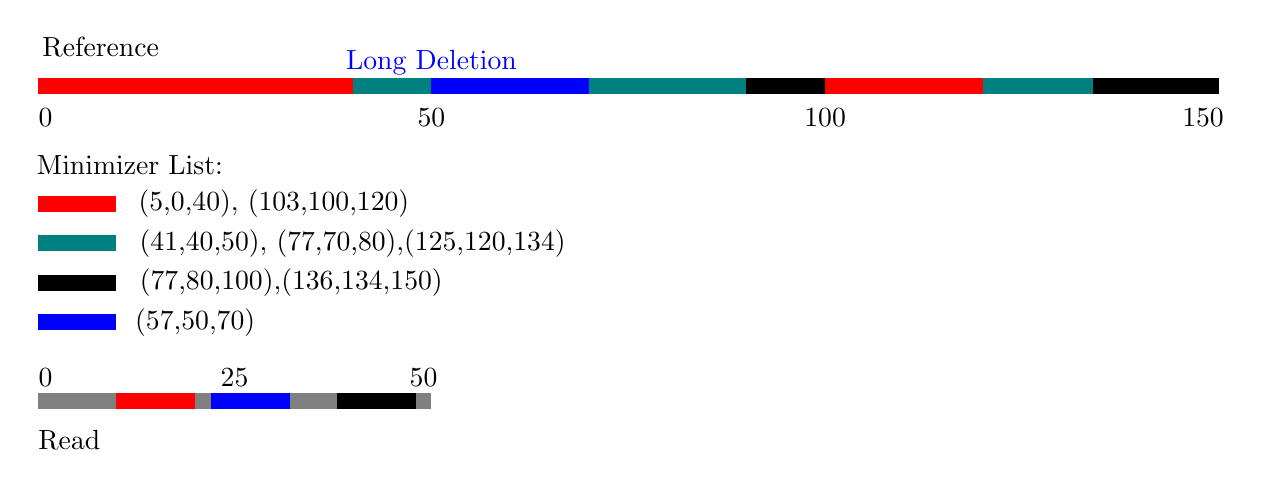
\begin{tikzpicture}[]
	
	%reference
	\draw[line width=2mm] (0,4) -- (15,4);
	\draw[line width=2mm,color=red] (0,4) -- (4,4);
	\draw[line width=2mm,color=green!50!blue] (4,4) -- (5,4);
	\draw[line width=2mm,color=blue] (5,4) -- (7,4);
	\draw[line width=2mm,color=green!50!blue] (7,4) -- (9,4);
	\draw[line width=2mm,color=red] (10,4) -- (12,4);
	\draw[line width=2mm,color=green!50!blue] (12,4) -- (13.4,4);
	%read
	\draw[line width=2mm,color=black!50] (0,0) -- (5,0);
	\draw[line width=2mm,color=red] (1,0) -- (2,0);
	\draw[line width=2mm,color=blue] (2.2,0) -- (3.2,0);
	\draw[line width=2mm,color=black] (3.8,0) -- (4.8,0);
	
	%others
	\draw[line width=2mm,color=red] (0,2.5) -- (1,2.5);
	\node[rectangle](refer) at (3,2.5) {(5,0,40), (103,100,120)};
	\draw[line width=2mm,color=green!50!blue] (0,2) -- (1,2);
	\node[rectangle](refer) at (4,2) {(41,40,50), (77,70,80),(125,120,134)};
	\draw[line width=2mm,color=black] (0,1.5) -- (1,1.5);
	\node[rectangle](refer) at (3.22,1.5) { (77,80,100),(136,134,150)};
	\draw[line width=2mm,color=blue] (0,1) -- (1,1);
	\node[rectangle](refer) at (2,1) { (57,50,70)};
	%labels
	\node[rectangle](refer) at (0.8,4.5) {Reference};
	\node[rectangle](refer) at (0.1,3.6) {0};
	\node[rectangle](refer) at (5,3.6) {50};
	\node[rectangle](refer) at (10,3.6) {100};
	\node[rectangle](refer) at (14.8,3.6) {150};
	\node[rectangle,color=blue](refer) at (5,4.3) {Long Deletion};
	\node[rectangle](refer) at (0.4,-0.5) {Read};
	\node[rectangle](refer) at (0.1,0.3) {0};
	\node[rectangle](refer) at (2.5,0.3) {25};
	\node[rectangle](refer) at (4.9,0.3) {50};
	\node[rectangle](refer) at (1.17,3) {Minimizer List:};
	%arrows
	%\draw[line width=1mm,color=black!50,->] (1.5,0.2) ..  controls (1.5,3.8) and (2.5,0.2) .. (2.5,3.8);
	%\draw[line width=1mm,color=black!50,->] (3.2,0.2) .. controls(3.2,3.8) and (8,0.2) .. (8,3.8);
	\end{tikzpicture}
	\caption{There are four distinct minimizer found in the reference which are showed with four different color. Their positions are listed with triplets (position of minimizer, starting position of the consecutive covered window, ending position of the consecutive covered window). In the read, we have found three minimizer among four. Grayed portion indicates that these minimizer are not found in the reference.In Naive Minimizer approach, mapping is done based on these information.} \label{fig:naive_min}
\end{figure}

\end{document}